\documentclass[UTF-8]{ctexart}
\usepackage{geometry}
\geometry{a4paper, margin=2cm}
\usepackage{graphicx}
\usepackage{longtable}
\usepackage{booktabs}
\usepackage{enumitem}
\usepackage{svg} 
\usepackage{float}

\begin{document}

\title{需求分析}
\author{}
\date{}
\maketitle
\newpage

\tableofcontents
\newpage

\section{简介}
\subsection{目的}
本文档旨在详细描述图书管理系统的功能需求、非功能需求、数据需求和实现方案，为系统开发和测试提供指导依据。

\subsection{名词定义}

\begin{longtable}{ll}
\toprule
名词 & 解释 \\
\midrule
ISBN & 国际标准书号，图书的唯一标识符 \\
借阅记录 & 记录图书借阅和归还信息的数据 \\
库存 & 图书的可用数量 \\
未归还 & 已借出但尚未归还的图书状态 \\
\bottomrule
\end{longtable}

\section{总体概述}
\subsection{软件概述}
图书管理系统是一款专为图书管理场景设计的软件系统，为用户提供图书信息管理和借阅流程跟踪的数字化工具，实现图书全生命周期管理和借阅业务的规范化、智能化处理。
系统设计简洁明了，功能完整，易于使用和维护，短小精悍，适合小型图书馆、学校图书室或个人图书收藏管理使用，为图书管理工作提供高效、便捷的数字化解决方案。

\subsection{软件功能}
本项目输出产品名称为图书管理系统，是一个用于管理图书和借阅流程的软件系统，在这个系统中将实现以下特性：
\begin{enumerate}[label=\arabic{enumi}、]
\item 支持图书信息的管理，包括新增、查询、修改、删除图书。 （优先级：重要）
\item 支持图书借阅流程管理，包括借阅图书、归还图书、查看借阅记录。 （优先级：重要）
\item 支持按多种方式查询图书，包括按书名、作者、ISBN查询。（优先级：重要）
\item 支持借阅记录的多维度查询，包括所有记录、指定借阅人记录、未归还记录。 （优先级：一般）
\item 支持数据的本地存储，保存图书和借阅记录数据。 （优先级：重要）
\item 提供图形化操作界面，满足不同场景的使用需求。 （优先级：一般）
\item 支持库存管理，自动处理借阅和归还时的库存变化。（优先级：一般）
\end{enumerate}

图书管理系统不支持以下特性： 
\begin{enumerate}[label=\arabic{enumi}、]
\item 不支持借阅期限和逾期处罚功能。 
\item 不支持图书预约功能。 
\end{enumerate}

向用户提供以下操作接口：
\begin{itemize}
\item 导航栏：首页、图书管理、借阅管理。
\item 图书管理页：图书搜索、图书列表、新增/修改/删除操作。
\item 借阅管理页：借阅/归还操作、借阅记录查询。
\item 首页：系统功能介绍。
\end{itemize}

\subsection{用户特征}
\begin{enumerate}[label=\arabic{enumi}]
\item 图书管理员 ：
\begin{itemize}
\item 角色：负责图书的采购、分类、编目等管理工作。
\item 特征：了解图书分类和编目知识，具备基本的计算机操作技能。
\item 需求：需要便捷的图书信息管理功能，能够快速录入和修改图书信息。
\end{itemize}

\item 系统维护人员 ：
\begin{itemize}
\item 角色：负责系统的安装、配置和维护。
\item 特征：具备基本的计算机技术知识。
\item 需求：需要系统稳定可靠，数据备份方便，易于维护和扩展。
\end{itemize}

\item 普通用户：
\begin{itemize}
\item 角色：查询图书信息和个人借阅记录。
\item 特征：具备基本的计算机操作能力。
\item 需求：需要简单直观的查询界面，能够快速找到所需图书信息。
\end{itemize}
\end{enumerate}

\subsection{可行性分析}
本项目为软件工程课程大作业，围绕图书管理系统的开发目标，从四大核心维度论证落地可行性。

\subsubsection{技术可行性}
系统基于Web和Python 开发，核心功能仅需 Python 标准库即可实现，扩展版本采用轻量开源框架，无技术壁垒；兼容 Windows、macOS、Linux 全主流操作系统，仅需普通个人电脑即可完成开发与运行，完全适配课程所学技术栈，开发落地无风险。 

\subsubsection{操作可行性}
系统采用直观的层级菜单与标准化图形界面设计，操作流程贴合图书管理实际业务场景，配套清晰的输入指引与友好的错误提示；目标用户仅需具备基础计算机操作能力即可快速上手，无需专业技术培训，使用门槛低。 

\subsubsection{经济可行性}
项目全流程零额外成本投入，所用开发工具、框架、依赖库均为开源免费资源，无版权、授权、硬件采购、运维等相关费用。

\subsubsection{进度可行性}
系统采用模块化拆分设计，核心业务逻辑清晰，可分模块开发与测试；整体开发周期短，项目进度完全可控。 

综上，本项目在技术、操作、经济、进度维度均具备完整的落地可行性，可正式启动开发工作。

\section{系统功能性分析}
\subsection{基于场景的建模}
系统将划分为三大核心功能模块：系统管理模块、借阅管理模块、图书管理模块，完整覆盖图书管理全业务流程的功能需求，同时识别了三类核心actor与其对应权限：

\subsubsection{总体用例图}

总体用例图（如图3.1.1所示）是面向用户视角的系统功能边界与角色交互核心模型，该图从用户视角出发，明确了系统的功能边界和各角色之间的交互关系，主要包含以下核心内容：
\begin{itemize}
\item 三大模块：系统管理模块、借阅管理模块、图书管理模块
\item 三类actor：图书管理员、系统维护人员、普通用户
\item 定义了各角色的操作权限和可用功能
\end{itemize}

\begin{figure}[H]
    \centering
    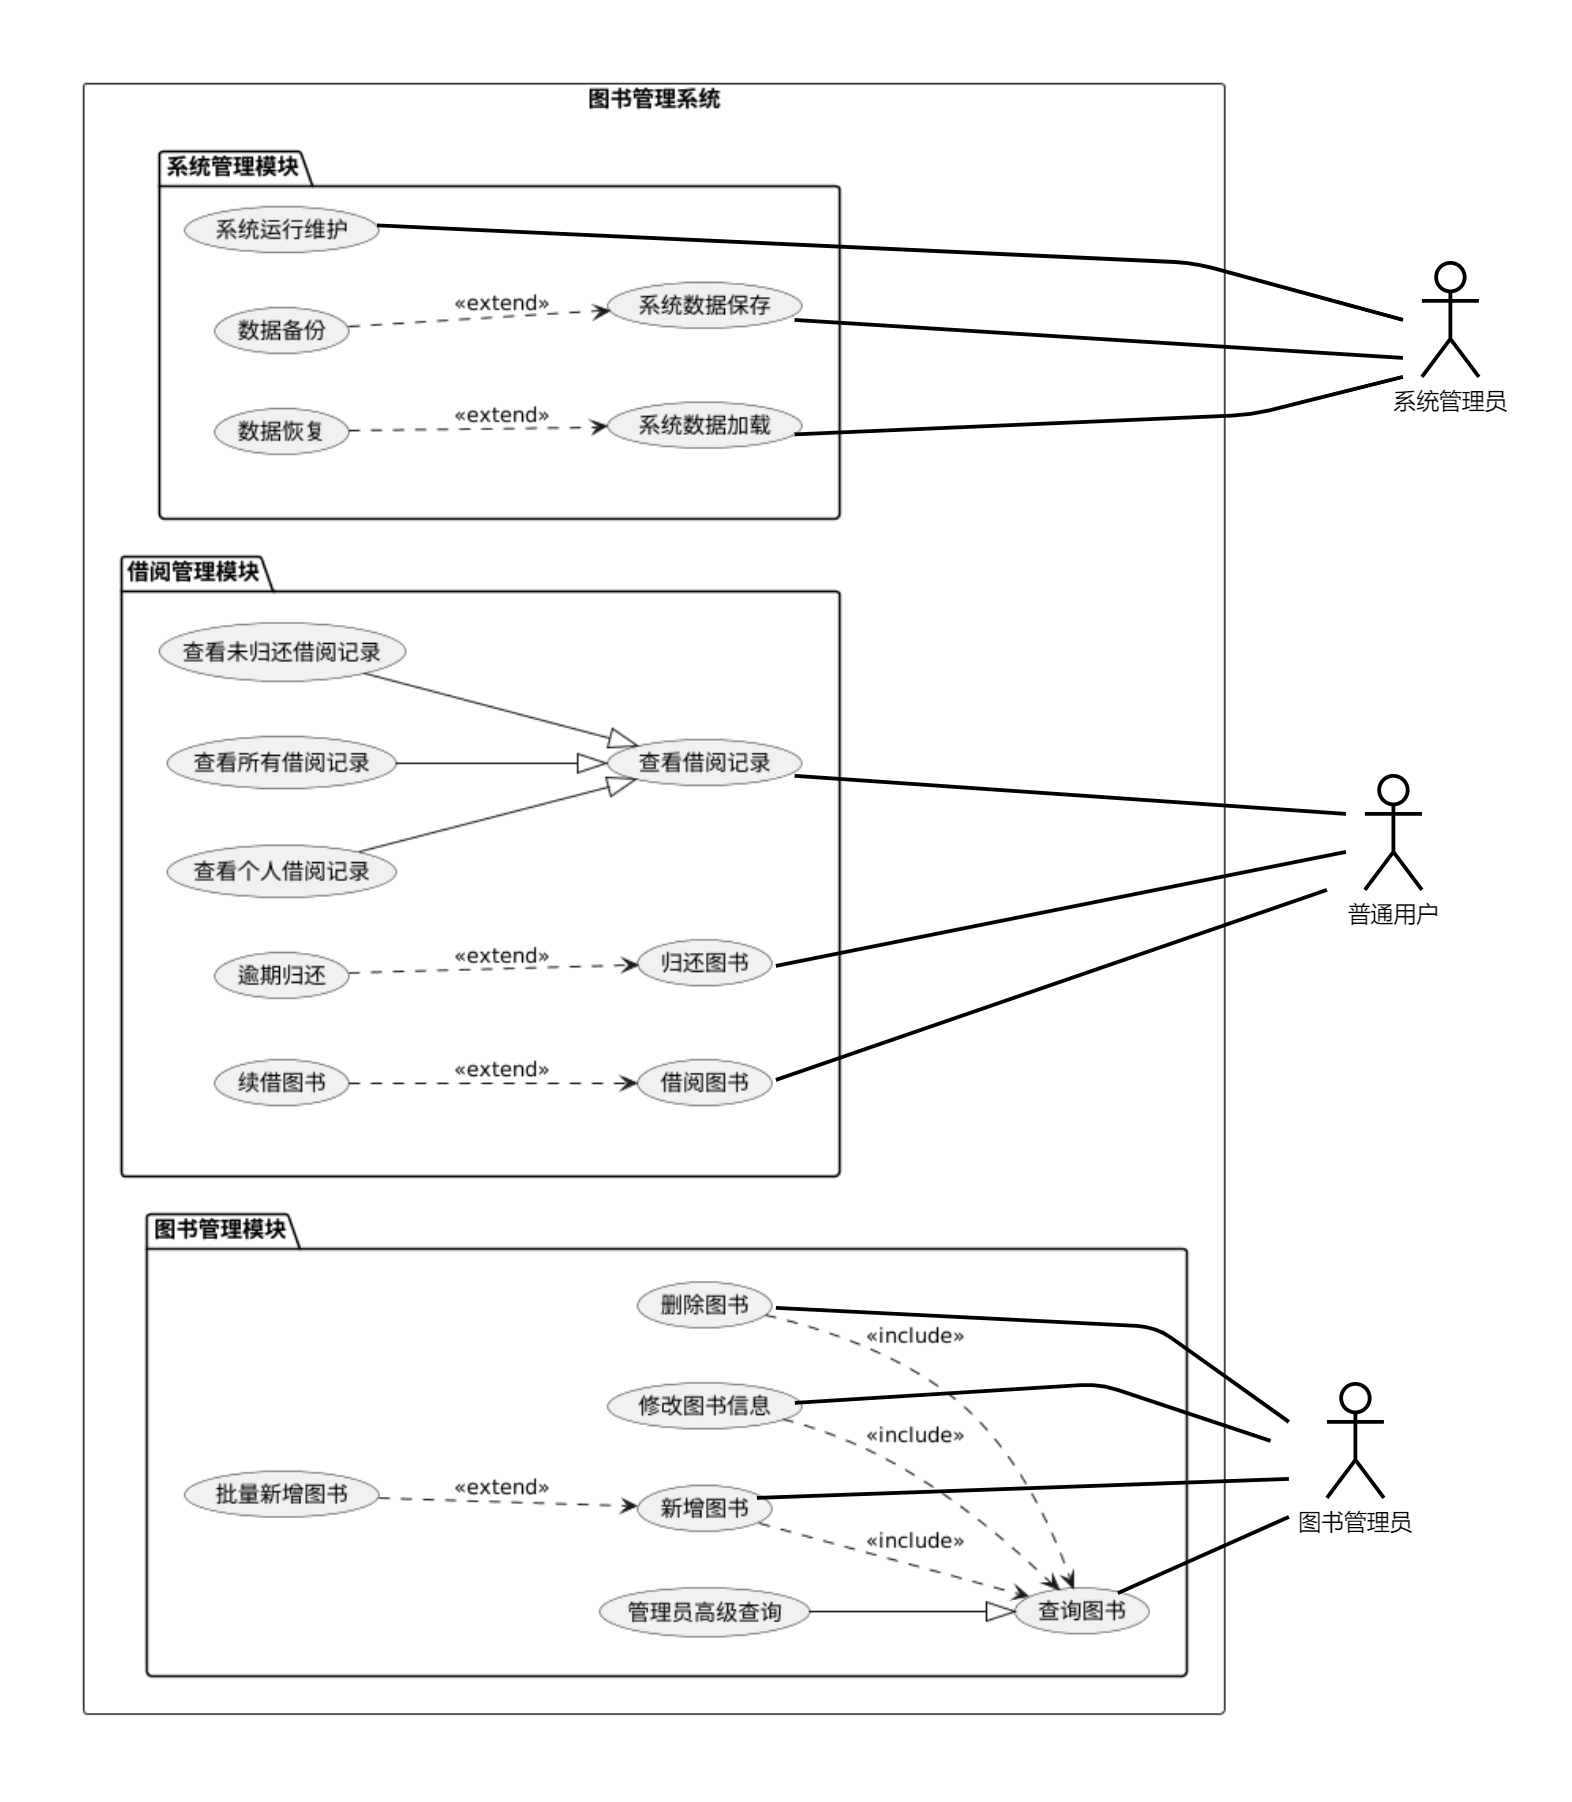
\includegraphics[width=0.8\textwidth]{sysytemActor.png}
    \caption{3.1.1 系统总体用例图}
\end{figure}

\subsubsection{总体泳道图}

总体泳道图（如图3.1.2所示）通过泳道划分不同管理模块与责任主体，清晰呈现系统业务流程中各参与方的职责边界、操作顺序与数据交互关系。

该图以泳道形式展示了系统业务流程的执行过程，主要特点包括：
\begin{itemize}
\item 按功能模块和责任主体划分泳道，明确职责边界
\item 展示了操作顺序和执行路径
\item 呈现了数据交互关系和信息传递方向
\item 反映了系统业务流程的整体架构和协作模式
\end{itemize}\vspace{2\baselineskip}
\begin{figure}[H]
    \centering
    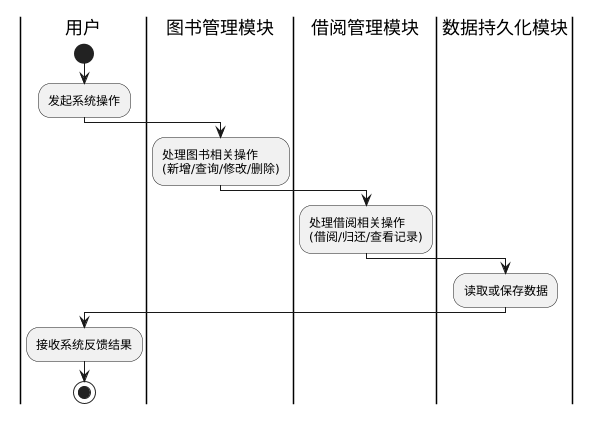
\includegraphics[width=0.6\textwidth,height=0.9\textheight,keepaspectratio]{SwimLane.png}
    \caption{3.1.2 总体泳道图}
\end{figure}

\vspace{3\baselineskip}
\subsubsection{总体活动图}

总体活动图（如图3.1.3所示）描述系统业务操作的执行流程、判断逻辑与分支走向，直观呈现用户操作从发起至结束的全流程处理规则。

该图详细展示了系统业务操作的执行过程，核心内容包括：
\begin{itemize}
\item 执行流程和步骤
\item 判断逻辑和分支走向
\item 发起至结束的全流程处理规则
\item 执行条件和结果
\end{itemize}

\begin{figure}[H]
    \centering
    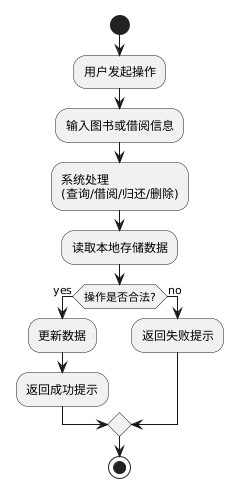
\includegraphics[width=0.7\textwidth, height=0.9\textheight, keepaspectratio]{SystemActivity.png}
    \caption{3.1.3 总体活动图}
\end{figure}


\subsubsection{子模块分析}
\paragraph{借阅图书用例及建模}
\leavevmode 
\begin{table}[H]
\centering
\begin{tabular}{|p{3cm}|p{12cm}|}
\hline
\textbf{用例描述} & 普通用户经过系统完成借阅操作，同步扣减图书库存、生成借阅记录 \\
\hline
\textbf{参与者} & 普通用户 \\
\hline
\textbf{前置条件} & 1. 普通用户已进入借阅管理模块；

2. 目标图书已在系统中存在，可通过 ISBN 定位；

3. 系统图书与借阅记录数据已正常加载 \\
\hline
\textbf{后置条件} & 1. 系统生成有效借阅记录，状态标记为 “未归还”；

2. 对应图书的库存数量扣减 1；

3. 借阅记录列表与图书库存同步更新 \\
\hline
\textbf{基本事件流} & 1. 普通用户进入借阅操作页面

2. 普通用户输入信息，提交借阅请求

3. 系统校验是否满足借阅条件

4. 所有校验通过，系统生成借阅记录，记录借阅时间、借阅人、图书 ISBN 等信息

5. 系统提示 ，更新借阅记录列表，完成操作 \\
\hline
\textbf{意外事件流} & 1. 若 ISBN 对应的图书不存在，系统提示 ，终止操作

2. 若图书库存为 0，系统提示 ，终止操作

3. 借阅人操作非法，系统提示 ，终止操作

4. 若数据保存失败，系统提示 ，回滚库存扣减与记录生成操作 \\
\hline
\textbf{活动图} & 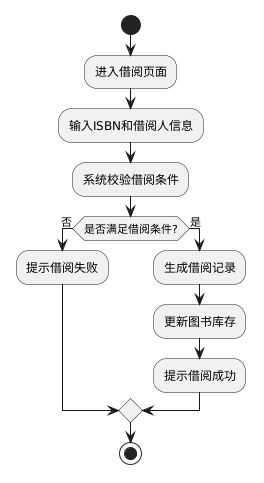
\includegraphics[width=0.7\textwidth, height=0.47\textheight, keepaspectratio]{BorrowBookActivity.png} \\
\hline
\end{tabular}
\setcounter{table}{0} 
\caption{借阅图书用例分析}
\end{table}

\paragraph{归还图书用例及建模}
\leavevmode 
\begin{table}[H]
\centering
\begin{tabular}{|p{3cm}|p{12cm}|}
\hline
\textbf{用例描述} & 普通用户办理图书归还手续，系统校验有效借阅记录后，完成归还操作 \\
\hline
\textbf{参与者} & 普通用户 \\
\hline
\textbf{前置条件} & 1. 普通用户已进入借阅管理模块；

2. 用户信息合法

3. 系统数据已正常加载 \\
\hline
\textbf{后置条件} & 1. 对应借阅记录更新归还时间，状态标记为 “已归还”；

2. 对应图书的库存数量增加 1；

3. 借阅记录列表与图书库存同步更新 \\
\hline
\textbf{基本事件流} & 1. 普通用户进入归还操作页面

2. 普通用户输入信息，提交归还请求

3. 系统查询匹配的、未归还的借阅记录，校验记录是否存在

4. 系统根据 ISBN 查询目标图书，校验图书是否存在

5. 校验通过，系统更新借阅记录的归还时间与状态

6. 系统提示 “图书归还成功”，更新借阅记录列表，完成操作 \\
\hline
\textbf{意外事件流} & 1. 若未找到匹配的未归还借阅记录，系统提示 ，终止操作

2. 若 ISBN 对应的图书不存在，系统提示 ，终止操作

3. 若数据更新失败，系统提示 ，回滚库存恢复与记录更新操作 \\
\hline
\textbf{活动图} & 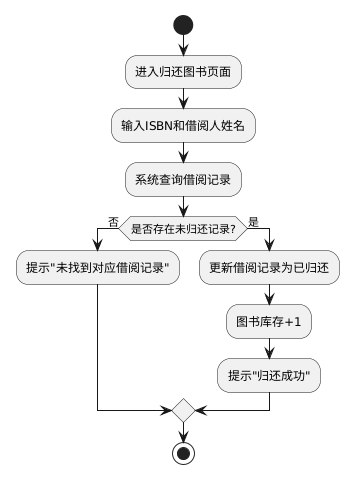
\includegraphics[width=0.7\textwidth, height=0.52\textheight, keepaspectratio]{ReturnBookActivity.png} \\
\hline
\end{tabular}
\caption{归还图书用例分析}
\end{table}

\paragraph{查看借阅记录用例及建模}
\leavevmode 
\begin{table}[H]
\centering
\begin{tabular}{|p{3cm}|p{12cm}|}
\hline
\textbf{用例描述} & 用户选择查看维度，系统筛选并展示对应的借阅记录，支持多场景的记录追溯 \\
\hline
\textbf{参与者} & 普通用户 \\
\hline
\textbf{前置条件} & 1. 用户已进入借阅管理模块；

2. 系统借阅记录与图书数据已正常加载 \\
\hline
\textbf{后置条件} & 系统展示匹配的借阅记录列表，无匹配结果时给出明确提示，不修改存储数据 \\
\hline
\textbf{基本事件流} & 1. 普通用户，进入记录查询页面

2. 普通用户选择查看维度，补充筛选条件，提交查询请求

3. 系统按筛选条件遍历借阅记录，匹配对应数据

4. 系统为每条记录匹配对应的图书书名，渲染借阅记录列表，完成操作 \\
\hline
\textbf{意外事件流} & 1. 若无匹配的借阅记录，系统提示 ，展示空列表

2. 若选择指定借阅人查询但未输入姓名，系统提示 ，终止查询

3. 若数据未加载完成，系统提示 ，终止查询 \\
\hline
\textbf{活动图} & 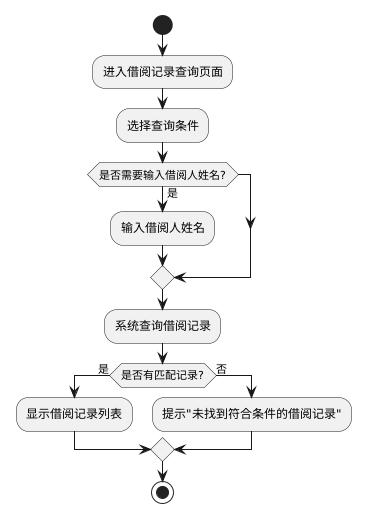
\includegraphics[width=0.7\textwidth, height=0.6\textheight, keepaspectratio]{RecordsViewActivity.png} \\
\hline
\end{tabular}
\caption{查看借阅记录用例分析}
\end{table}

\paragraph{查询图书用例分析及建模}
\leavevmode 
\begin{table}[H]
\centering
\begin{tabular}{|p{3cm}|p{12cm}|}
\hline
\textbf{用例描述} & 用户选择查询维度，输入关键词检索图书信息，系统返回匹配的图书列表，是所有图书操作的前置基础能力 \\
\hline
\textbf{参与者} & 普通用户 \\
\hline
\textbf{前置条件} & 1. 用户已进入系统，图书管理模块可正常访问；

2. 系统图书数据已完成加载 \\
\hline
\textbf{后置条件} & 1. 系统展示匹配的图书列表，无匹配结果时给出明确提示；

2. 不修改系统任何存储数据 \\
\hline
\textbf{基本事件流} & 1. 用户进入图书管理模块，进入查询功能页面

2. 用户选择查询方式

3. 用户输入查询关键词，提交查询请求

4. 系统根据查询维度与关键词，遍历图书数据执行匹配

5. 系统渲染匹配的图书列表，完成查询操作 \\
\hline
\textbf{意外事件流} & 1. 若关键词为空，系统提示 ，终止查询

2. 若无匹配的图书数据，系统提示 ，展示空列表

3. 若系统数据未加载完成，系统提示 ，终止查询 \\
\hline
\textbf{活动图} & 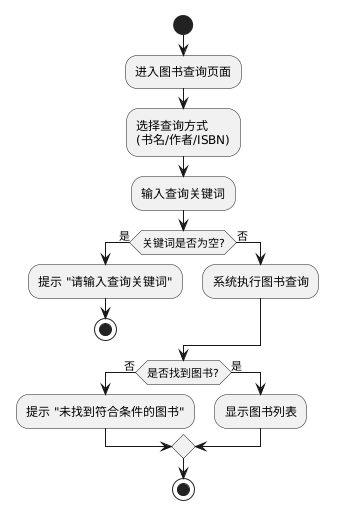
\includegraphics[width=0.7\textwidth, height=0.58\textheight, keepaspectratio]{QueryBookActivity.png} \\
\hline
\end{tabular}
\caption{查询图书用例分析}
\end{table}

\paragraph{新增图书用例分析及建模}
\leavevmode 
\begin{table}[H]
\centering
\begin{tabular}{|p{3cm}|p{12cm}|}
\hline
\textbf{用例描述} & 图书管理员录入图书基础信息，系统校验 ISBN 唯一性后，完成图书入库与信息存储 \\
\hline
\textbf{参与者} & 图书管理员 \\
\hline
\textbf{前置条件} & 1. 管理员已进入图书管理模块，拥有图书操作权限；

2. 系统数据已正常加载完成 \\
\hline
\textbf{后置条件} & 1. 图书信息成功写入系统本地存储；2. 图书库存同步更新；

3. 图书列表自动刷新，展示新增数据 \\
\hline
\textbf{基本事件流} & 1. 管理员点击“新增图书”入口，进入信息录入页面

2. 管理员录入图书必填信息

3. 系统校验并通过，系统将图书信息写入本地存储

4. 系统提示，刷新图书列表，完成操作 \\
\hline
\textbf{意外事件流} & 1. 若 ISBN 已存在，返回信息，终止操作，保留已录入信息

2. 若必填项为空，返回提示，终止提交

3. 若库存输入为负数，返回提示，终止提交

4. 若数据存储失败，返回提示，回滚操作 \\
\hline
\textbf{活动图} & 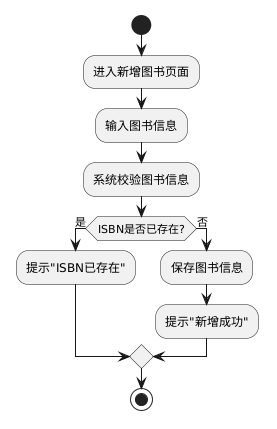
\includegraphics[width=0.7\textwidth, height=0.57\textheight, keepaspectratio]{AddBookActivity.png} \\
\hline
\end{tabular}
\caption{新增图书用例分析}
\end{table}

\paragraph{修改图书信息用例分析及建模}
\leavevmode 
\begin{table}[H]
\centering
\begin{tabular}{|p{3cm}|p{12cm}|}
\hline
\textbf{用例描述} & 图书管理员对已入库的图书信息进行编辑更新，系统校验后完成数据修改，必须先通过查询定位目标图书 \\
\hline
\textbf{参与者} & 图书管理员 \\
\hline
\textbf{前置条件} & 1. 管理员已通过查询功能定位到目标图书；

2. 系统数据已正常加载完成 \\
\hline
\textbf{后置条件} & 1. 目标图书的信息在存储中完成更新；

2. 图书列表同步刷新，展示最新信息 \\
\hline
\textbf{基本事件流} & 1. 管理员在图书查询结果中，进行修改

2. 系统回显该图书的当前信息，进入编辑页面

3. 管理员修改图书信息

4. 管理员提交修改，系统校验修改后信息的合法性

5. 校验通过，系统更新存储中的图书数据

6. 系统提示，刷新图书列表，完成操作 \\
\hline
\textbf{意外事件流} & 1. 若修改后的库存为负数，系统提示 ，终止提交

2. 若必填项修改为空，系统提示 ，终止提交

3. 若数据更新失败，系统提示 ，回滚数据，保留原信息 \\
\hline
\textbf{活动图} & 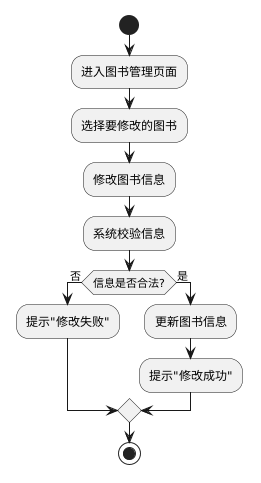
\includegraphics[width=0.7\textwidth, height=0.56\textheight, keepaspectratio]{ChangeBookActivity.png} \\
\hline
\end{tabular}
\caption{修改图书信息用例分析}
\end{table}

\paragraph{删除图书用例及建模}
\leavevmode 
\begin{table}[H]
\centering
\begin{tabular}{|p{3cm}|p{12cm}|}
\hline
\textbf{用例描述} & 图书管理员对目标图书执行下架删除操作，系统校验无未归还借阅记录后完成删除，必须先通过查询定位目标图书 \\
\hline
\textbf{参与者} & 图书管理员 \\
\hline
\textbf{前置条件} & 1. 管理员已通过查询功能定位到目标图书；

2. 系统借阅记录数据已正常加载 \\
\hline
\textbf{后置条件} & 1. 目标图书从系统存储中永久移除；

2. 图书列表同步刷新，移除该条数据 \\
\hline
\textbf{基本事件流} & 1. 管理员在图书查询结果中，进行删除 

2. 系统弹出二次确认弹窗，提示管理员确认删除操作

3. 管理员确认删除，系统校验该图书是否存在未归还的借阅记录

4. 校验无未归还记录，系统从存储中删除该图书数据

5. 系统提示，刷新图书列表，完成操作 \\
\hline
\textbf{意外事件流} & 1. 若该图书存在未归还的借阅记录，系统提示 "该图书有未归还的借阅记录"，终止操作

2. 若管理员取消确认，系统终止删除操作，保留原数据，并返回消息 

3. 若数据删除失败，系统提示,"数据删除失败" ，保留原数据 \\
\hline
\textbf{活动图} & 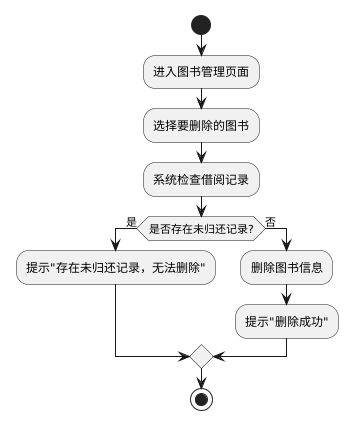
\includegraphics[width=0.7\textwidth, height=1.2\textheight, keepaspectratio]{DeleteBookActivity.png} \\
\hline
\end{tabular}
\caption{删除图书用例分析}
\end{table}







\subsection{面向数据流建模}
\subsubsection{数据流图}

数据流图（如图3.2.1所示）呈现了系统的数据边界与数据流转链路，识别了以下核心元素：

\begin{enumerate}
\item \textbf{外部实体}：数据的发起方与接收方，包括普通用户、图书管理员、系统管理员三类角色
\item \textbf{核心数据加工过程}：系统对数据的处理逻辑单元，对应系统的核心业务逻辑处理环节
\item \textbf{核心数据存储}：系统的持久化数据载体
\end{enumerate}
\vspace{1\baselineskip}
\textbf{核心数据流向}：
\begin{itemize}
\item 普通用户发起请求，系统获取图书数据，最终向用户返回操作结果与数据信息
\item 图书管理员发起请求，系统对本地书籍数据存储中的数据进行维护更新，向管理员返回操作结果
\item 系统管理员发起请求，系统对本地存储的全量数据进行管理与维护
\end{itemize}
\vspace{2\baselineskip}
\begin{figure}[H]
    \centering
   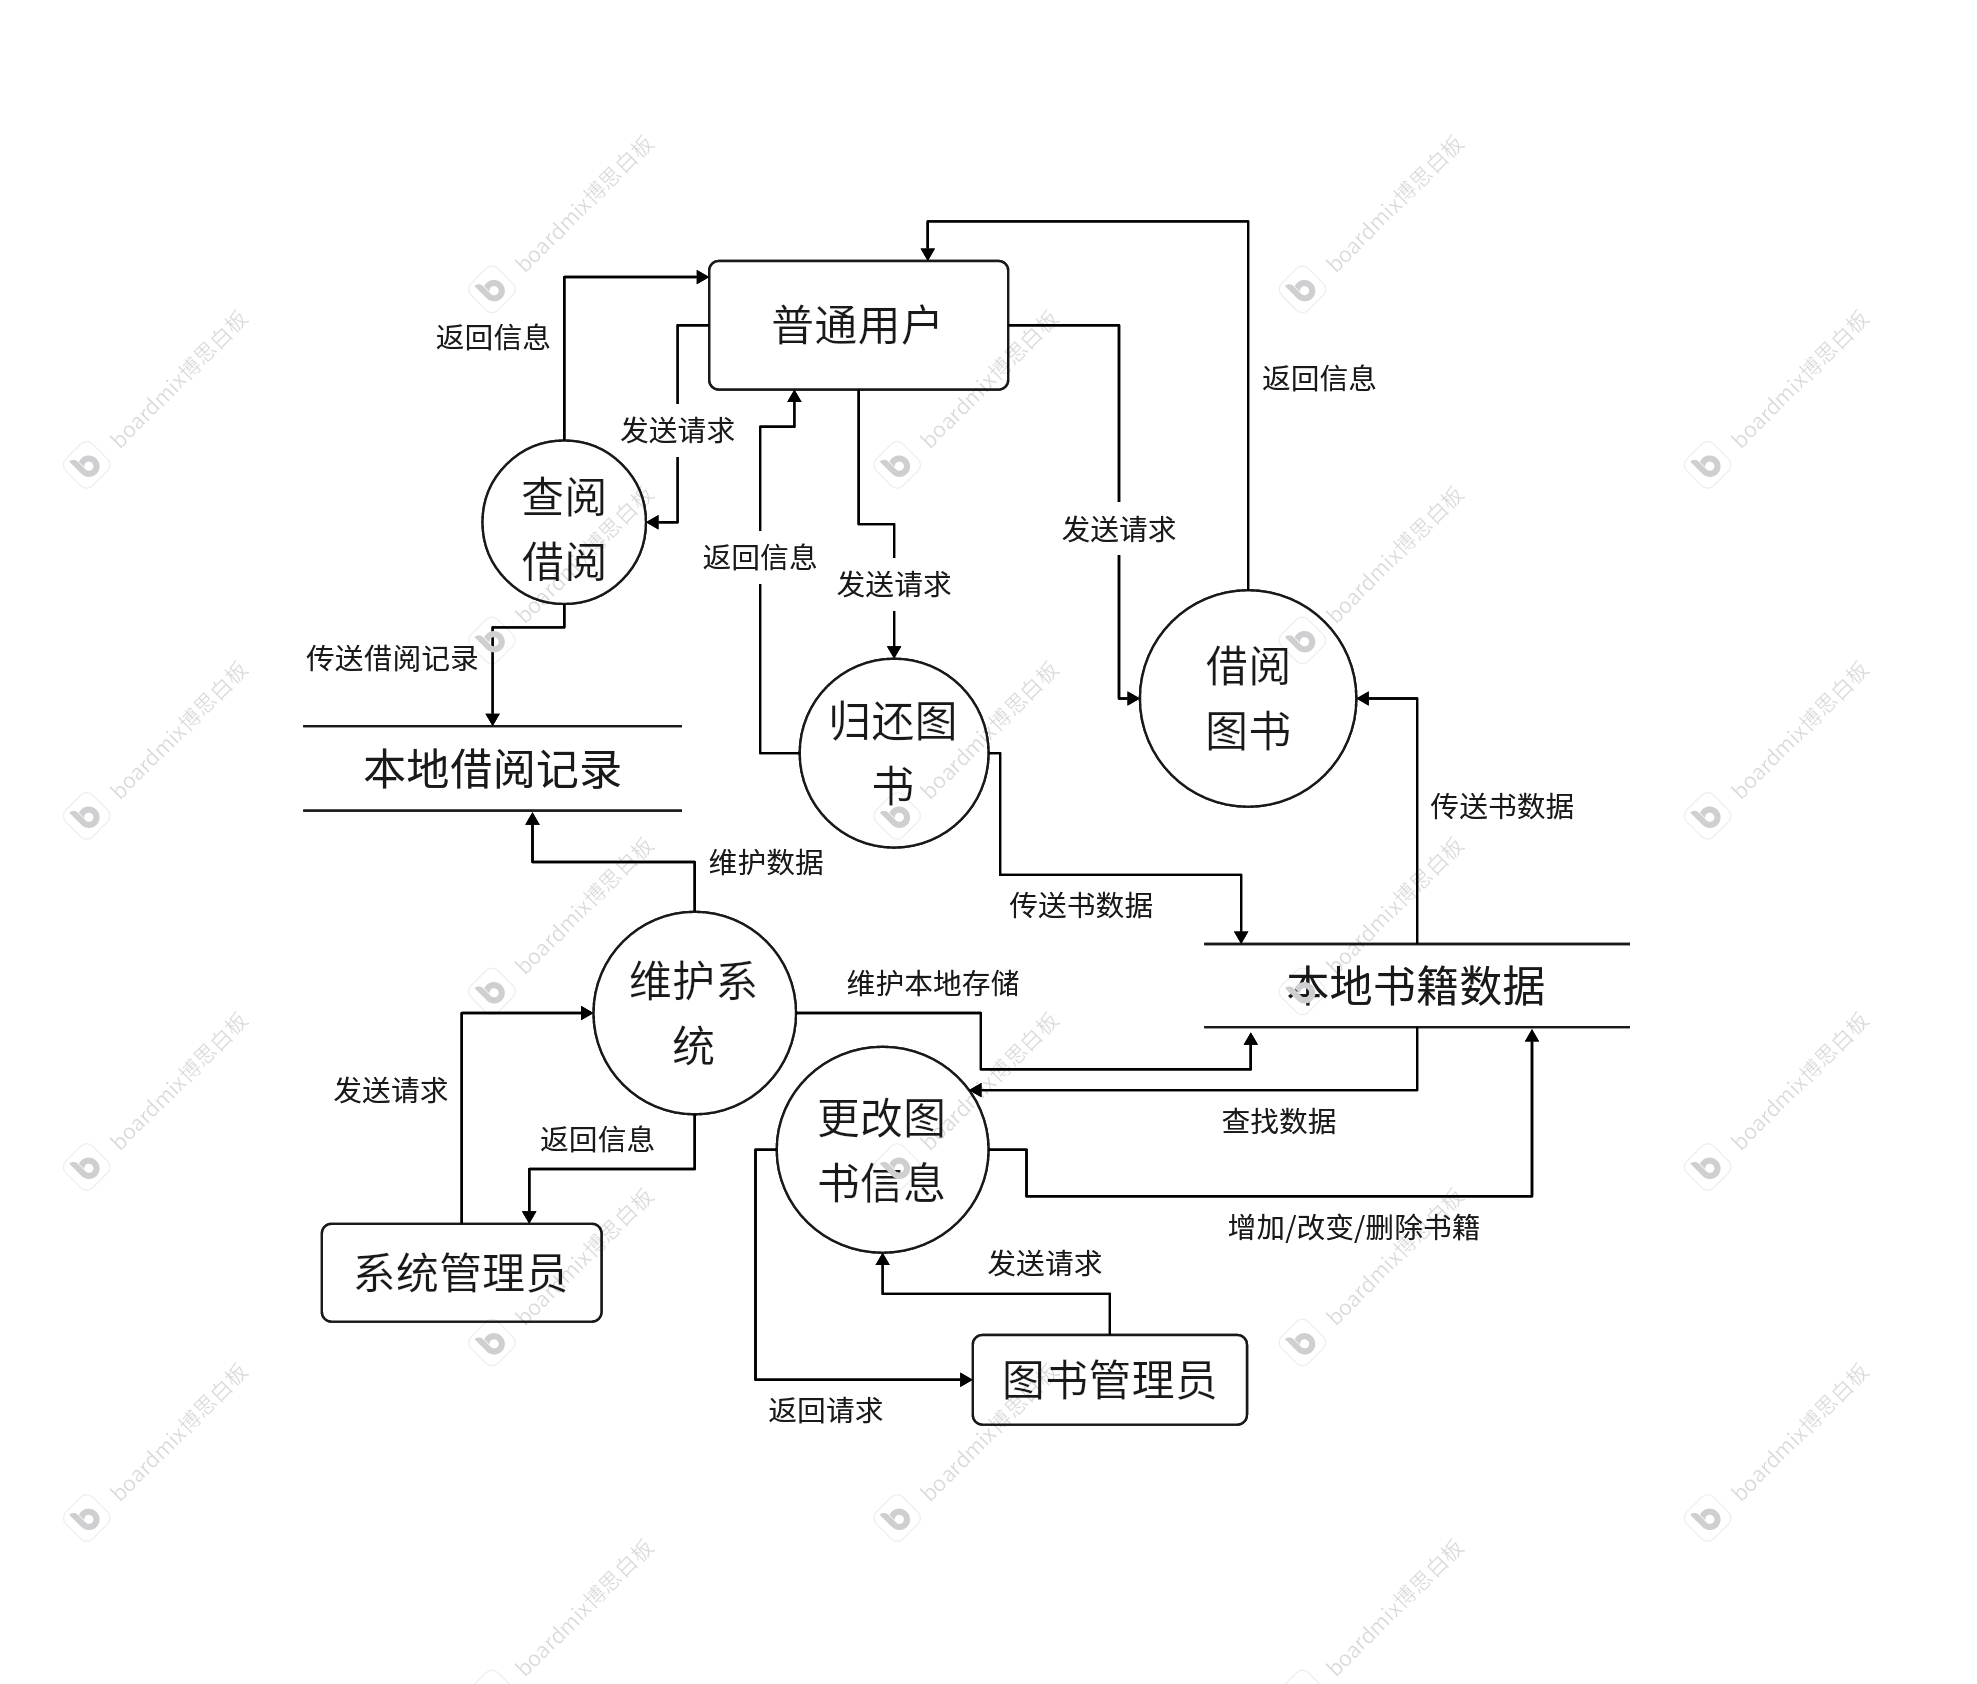
\includegraphics[width=0.9\textwidth, keepaspectratio]{DataFlowDiagram.png}
    \caption{3.2.1 系统数据流图}
\end{figure}

\newpage
\subsubsection{控制流图}
控制流图（如图3.2.2所示）描述系统程序运行时的控制流向、状态切换与模块调用关系，直观呈现系统从启动到退出的全生命周期运行逻辑。

控制流图完整覆盖了系统程序的运行状态，核心元素与控制流向如下：

\begin{enumerate}
\item \textbf{初始状态 Idle}：用户进入系统后，程序进入空闲等待状态，等待用户输入操作指令，是系统程序的初始状态与稳态
\item \textbf{核心处理单元}：
  \begin{itemize}
  \item Input 单元：接收用户输入各类核心输入数据
  \item Process 单元：程序的核心逻辑处理单元，划分为两大子模块
  \item Output 单元：输出程序的各类输出单元等
  \end{itemize}
\item \textbf{核心控制分支}：不同用户选择不同分支；完成操作后，可返回主界面，重新进入 Idle 等待状态，形成闭环控制；退出系统分支则直接结束程序运行
\item \textbf{数据持久化环节 SaveData}：所有涉及数据修改的操作，将更新后的数据写入本地存储。
\end{enumerate}

\begin{figure}[H]
    \centering
    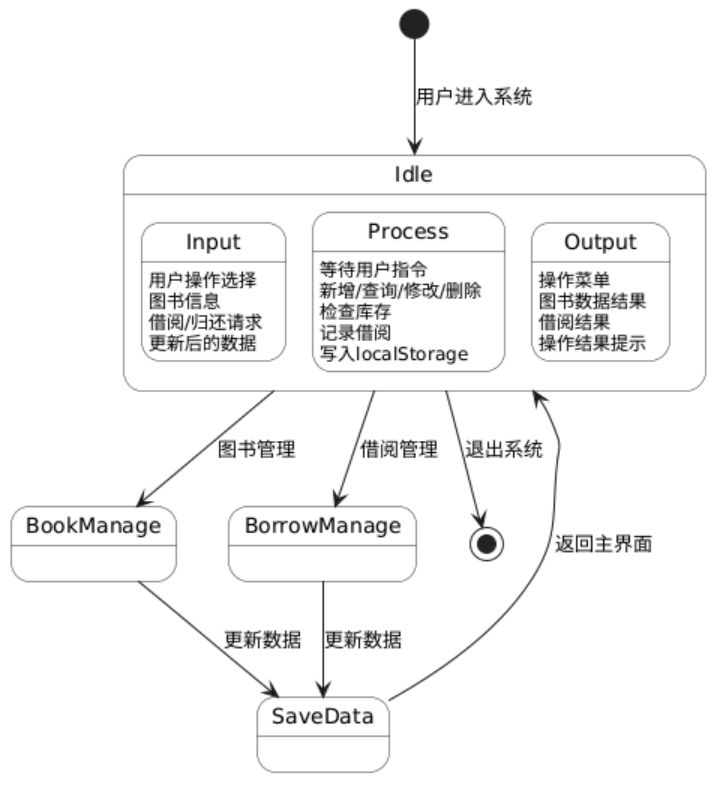
\includegraphics[width=0.8\textwidth]{ControlFlowDiagram.png}
    \caption{3.2.2 系统控制流图}
\end{figure}

\newpage
\subsection{面向类建模}
\subsubsection{类包分析}

类包分析图（如图3.3.1所示），遵循高内聚、低耦合的面向对象设计原则绘制，描述系统的代码分层架构、类的组织方式与包之间的依赖关系。

系统划分为5个核心包，每个包内包含对应的核心类，明确了包之间的依赖关系与协作逻辑：

\begin{enumerate}
\item \textbf{业务实体包（Entities）}：系统的核心领域层包，业务数据的载体，包含图书类（Book）、借阅记录类（BorrowRecord）2个核心实体类，封装了图书与借阅记录的核心属性与基础行为，被其他所有包依赖
\item \textbf{业务管理包（Managers）}：系统的业务逻辑层包，核心业务规则的执行单元，包含图书管理器（BookManager）、借阅管理器（BorrowManager）2个核心类，分别封装了图书管理、借阅管理的全量业务逻辑，依赖业务实体包、本地数据存储包、业务规则包
\item \textbf{本地数据存储包（LocalPersistence）}：系统的数据访问层包，负责数据的持久化读写操作，包含核心的本地存储类（LocalStorage），封装了本地数据的读写更新操作，为业务层提供统一的数据访问接口，依赖业务实体包
\item \textbf{业务规则包（SystemRules）}：系统的规则校验层包，封装了系统的核心业务规则与校验逻辑，包含借阅规则类（BorrowRule）、库存规则类（StockRule）2个核心类，为业务逻辑层提供统一的规则校验服务
\end{enumerate}

本类包分析图完整呈现了系统的分层架构与面向对象设计结构，明确了各层的职责边界与依赖关系。
\begin{figure}[H]
    \centering
    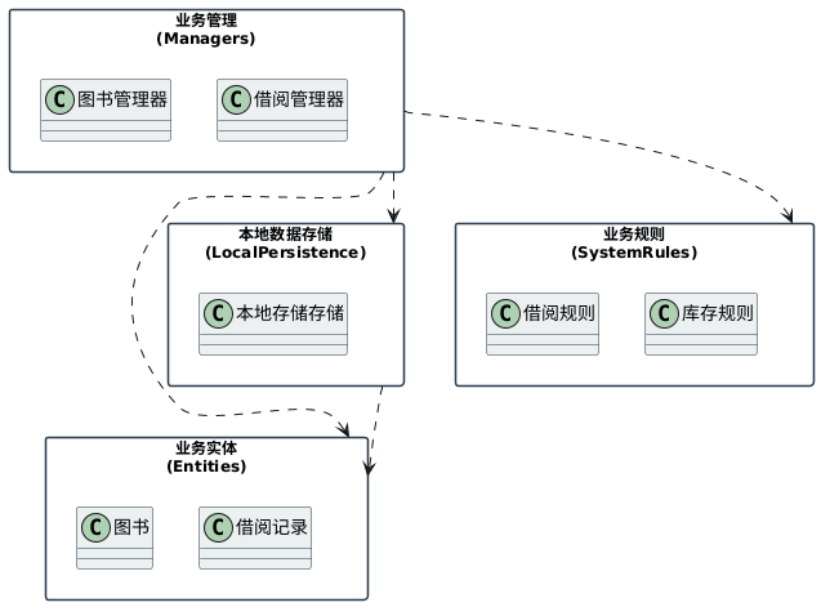
\includegraphics[width=0.8\textwidth]{PackageAnalysis.png}
    \caption{3.3.1 系统类包分析图}
\end{figure}

\newpage
\subsection{行为建模}
\subsubsection{状态图}

状态图（如图3.4.1所示）是描述图书对象在系统全生命周期中的状态变化、触发事件与转换规则。

\begin{enumerate}
\item \textbf{核心状态定义：}
  \begin{itemize}
  \item 可用状态：图书已入库、库存数量大于0，可被正常借阅的初始稳态
  \item 借阅中状态：图书已被借出、尚未归还的临时状态，不可被再次借阅
  \item 删除中状态：图书管理员发起删除操作后，系统正在校验删除条件的过渡状态
  \end{itemize}

\item \textbf{核心状态转换规则：}
  \begin{itemize}
  \item 可用→借阅中：触发事件为「借阅」操作
  \item 借阅中→可用：触发事件为「归还」操作
  \item 可用→删除中：触发事件为「删除图书」操作
  \item 删除中→删除成功：系统完成删除校验，执行图书数据删除操作
  \end{itemize}
\end{enumerate}

状态图完整定义了图书对象的全生命周期状态流转规则，为代码提供了标准化参考。

\begin{figure}[H]
    \centering
    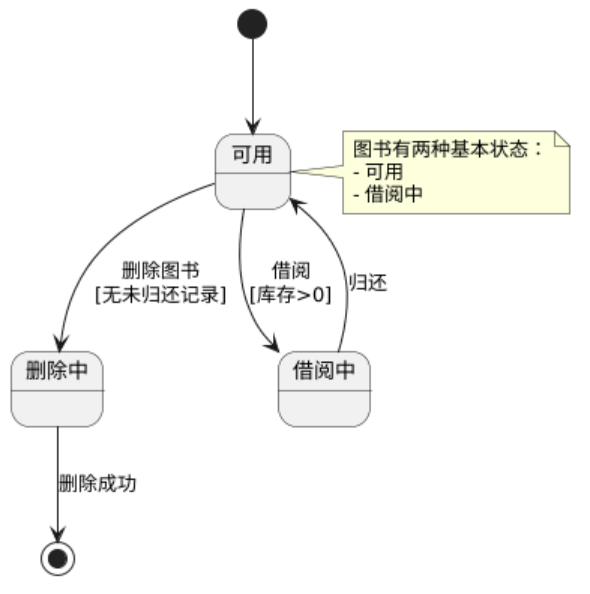
\includegraphics[width=0.8\textwidth]{BookState.png}
    \caption{3.4.1 系统书籍状态图}
\end{figure}

\newpage
\subsubsection{时序图}

时序图（如图3.4.2所示）是描述了对象之间的交互流程，按照时间顺序呈现消息发送与接收。

\begin{enumerate}
\item \textbf{核心交互对象：}用户、图书管理系统、本地存储

\item \textbf{核心业务场景：}
  \begin{itemize}
  \item 图书查询
  \item 新增图书
  \item 借阅图书
  \item 归还图书
  \end{itemize}
\end{enumerate}

时序图清晰呈现了各核心业务场景的对象交互流程，为代码提供了直接参考。

\begin{figure}[H]
    \centering
    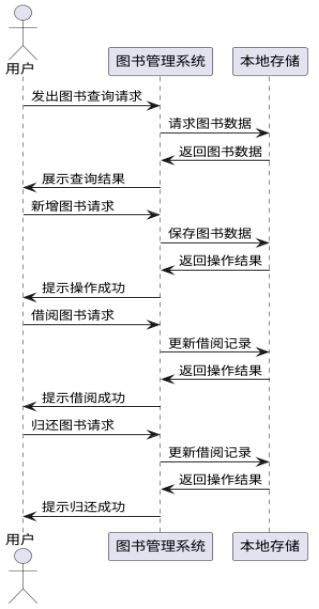
\includegraphics[width=0.8\textwidth,height=0.7\textheight,keepaspectratio]{Sequence.png}
    \caption{3.4.2 系统书籍时序图}
\end{figure}


\section{技术环境}
\subsection{硬件环境}
Intel Core i3 或同等性能处理器，内存4GB 及以上，有100MB 及以上可用空间。

\subsection{软件环境}
操作系统为Windows 7/10/11，macOS，Linux，Python版本Python 3.6 及以上。

\end{document}